\subsection{Discovering Microstrip Magic!}

\begin{tcolorbox}[colback=gray!10, colframe=black, title=E9F05] 

What is microstrip? 

\begin{enumerate}[label=\Alph*]
    \item Special shielding material designed for microwave frequencies
    \item Miniature coax used for low power applications
    \item Short lengths of coax mounted on printed circuit boards to minimize time delay between microwave circuits
    \item \textbf{Precision printed circuit conductors above a ground plane that provide constant impedance interconnects at microwave frequencies}
\end{enumerate} \end{tcolorbox}

\subsubsection{Related Concepts}

Microstrip technology is an essential aspect of modern microwave engineering and communication technologies. It involves the use of printed circuit board (PCB) techniques to create transmission lines that efficiently transmit microwave signals while maintaining a consistent impedance. This is crucial in minimizing signal reflections and ensuring signal integrity across various components in a microwave system.

A microstrip consists of a narrow conductor, usually made of copper, that is printed on a dielectric substrate. This conductor is situated above a ground plane, thereby forming a transmission line. The distance between the conductor and the ground plane, as well as the dimensions of the conductor itself, plays a critical role in determining the microstrip's characteristic impedance.

To understand microstrip design, one should be familiar with the following important concepts:

1. \textbf{Transmission Lines:}: These are specialized conductors that carry alternating current (AC) signals, particularly at high frequencies (microwave and RF).
2. \textbf{Impedance Matching:}: The process of ensuring that the impedance of the device matches that of the transmission line to minimize reflections.
3. \textbf{Dielectric Materials:}: The selection of an appropriate substrate material is essential for the performance of the microstrip. Different materials have various dielectric constants which will affect signal speed and attenuation.

\subsubsection{Calculation of Characteristic Impedance}

The characteristic impedance \( Z_0 \) of a microstrip can be approximated using the following formula:

\[
Z_0 = \frac{1}{2\pi} \sqrt{\frac{L}{C}}
\]

Where:
- \( L \) is the inductance per unit length
- \( C \) is the capacitance per unit length

To estimate \( Z_0 \) for a given microstrip design, we will often use the following simplified equation which assumes the width \( W \) of the microstrip conductor and the thickness \( h \) of the dielectric substrate:

\[
Z_0 \approx \frac{Z_{0,0}}{K}
\]

Where \( K \) is a correction factor based on the width-to-height ratio.

Assuming a microstrip with a width to height ratio of 1 and using experimentally determined coefficients, we can calculate the characteristic impedance.

\subsubsection{Diagram of Microstrip Configuration}

Below is a simple diagram using TikZ to illustrate a microstrip structure.

\begin{center}
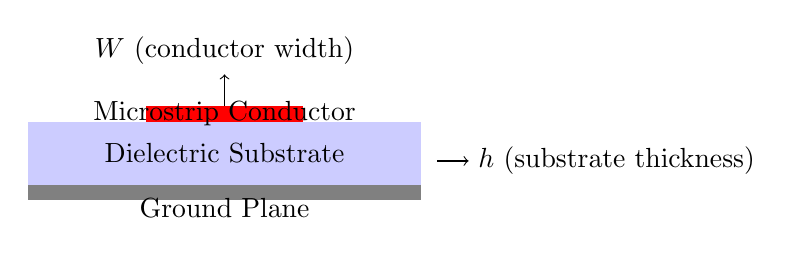
\begin{tikzpicture}
    % Draw the ground plane
    \fill[gray] (0,0) rectangle (5,0.2);
    \node at (2.5,-0.1) {Ground Plane};
    
    % Draw the dielectric substrate
    \fill[blue!20] (0,0.2) rectangle (5,1);
    \node at (2.5,0.6) {Dielectric Substrate};
    
    % Draw the microstrip conductor
    \fill[red] (1.5,1) rectangle (3.5,1.2);
    \node at (2.5,1.1) {Microstrip Conductor};
    
    % Draw dimensions
    \draw[->] (5.2,0.5) -- (5.6,0.5) node[right] {$h$ (substrate thickness)};
    \draw[->] (2.5,1.2) -- (2.5,1.6) node[above] {$W$ (conductor width)};
\end{tikzpicture}
\end{center}

Through understanding the properties of microstrip transmission lines and using the relevant calculations, one can effectively design and optimize microwave circuits that utilize this technology.